\chapter{Mathematical Framework for Sybil Attack Gain}
\label{chap:Sybil Attack Gain}
\noindent{}The point behind a sybil attack was to artificially increase one's accounting values in an attempt to subvert the reputation mechanism and obtain more data than one is actually entitled to. We then say that a Sybil attack is beneficial if the attacking agent or one of its sybils is chosen to receive some work when without the attack it would not have been. There's 4 ways of how this may be the case.\vspace{1em}\\ 

\begin{definition}[Beneficial Attacks]
\label{def:Beneficial Attacks}
\noindent{}A sybil attack by agent $j$ is considered beneficial if for some agent $i$ with choice set $C_i$, subjective work graph $G_i$, accounting mechanism $S_i^M$ and allocation policy $A_i$ that would pick some agents $A_i(S_i^M(G_i),C_i)\subset{}C_i$, we obtain one of 4 outcomes 
\begin{itemize}
\item[$\cdot$] j's score is increased such that $j\in{}A_i(S^M(G'_i),C'_i)$ when before $j\not\in{}A_i(S^M(G_i),C_i)$
\item[$\cdot$] Other agents' scores are lowered such that $j\in{}A_i(S^M(G'_i),C'_i)$ when before $j\not\in{}A_i(S^M(G_i),C_i)$
\item[$\cdot$] A sybil $s$ is assigned a score such that $s\in{}A_i(S^M(G'_i),C'_i)$ when before $s\not\in{}A_i(S^M(G_i),C_i)$
\item[$\cdot$] Other agents' scores are lowered such that $s\in{}A_i(S^M(G'_i),C'_i)$ for some sybil $s$ when before $s\not\in{}A_i(S^M(G_i),C_i)$. \vspace{1em}\\
\end{itemize}
\end{definition}
\noindent{}However, the upper conditions may be satisfied for a single attacking node, or for several. They may also hold true for multiple nodes $i$ from which the attacking agents could leech. Additionally, one or more of them may also still be satisfied after one or more of the attackers have received some work. \vspace{1em}\\

\noindent{}Hence, we see that some sybil attacks may be more beneficial than others depending on how much more work the attacker can consume than they were actually entitled to before the attack occurred. The upper definition is therefore rather inaccurate as it does not capture \textit{how} beneficial an attack is. \vspace{1em}\\


\section{Determining Cost \& Profit of Sybil Attacks}
\label{sec:Cost & Profit of Sybil Attacks}
\noindent{}We now want to introduce an exact definition of {\it how} beneficial a sybil attack is, which will be determined by the ratio of the work invested into the attack and the amount of work that the attacker(s) can gain through it. Seuken \& Parkes (2014) introduce the following definition of Sybil attack profit. \vspace{1em}\\

\begin{definition}[Sybil Attack Benefit]\ \\
\label{def:Sybil Attack Benefit}
\noindent{}Let $j$ be a malicious node perpetrating a sybil attack $\sigma_j^n$ on the work graph $G$, resulting in work graph $G'$. Here $n$ is variable. Now let $\omega_{-}^{n}>0$ denote the amount of work $j$ has invested into the sybil attack $\sigma_j^n$ and let $\omega_{+}^n$ be the amount of work that $j$ and its sybils can consume after the attack has been carried out as a result of it. Then $\sigma_j^n$ is called

\begin{itemize}
\item[] {\bf Strongly Beneficial} if $\omega^n_{+}>0$ and $\omega^n_{-}=0$ or if $\lim\limits_{n\rightarrow\infty}\frac{\omega^n_{+}}{\omega^n_{-}}=\infty$,
\item[] {\bf Weakly Beneficial} if $\omega^n_{+}>0$ and $\omega^n_{-}>0$ and $\exists c>0:\,\,\lim\limits_{n\rightarrow\infty}\frac{\omega^n_{+}}{\omega^n_{-}}\geq{}c$.
\end{itemize}
\end{definition}

\noindent{}It's almost impossible to prevent weakly beneficial sybil attacks from happening. Even though they might seem problematic they actually, if scaled, require an attacker to invest infinite resources in order to obtain infinite resources. A strongly beneficial sybil attack is much more fatal, seeing as an attacker can leech infinite resources without contributing a proportionate amount. This can bring an entire network to a stand-still and is therefore much more important to prevent than weakly beneficial sybil attacks. While it may be nice to find some upper bound for the value of $c$ in the definition above, it will be our goal to prevent strongly beneficial sybil attacks. \vspace{1em}\\

\noindent{}While the values for $\omega^n_{-}$ and $\omega^n_{+}$ may be intuitively clear, we realise that the more one thinks about them, the more involved these definitions actually turn out to be. In the existing literature, they have been introduced as above without any further explanation. In this chapter we aim to refine this definition and determine more rigorous definitions for the cost and profit of sybil attacks. For the value $\omega^n_{-}$ this is not so difficult, while $\omega^n_{+}$ is much less clear. We begin by introducing the cost or investment of a sybil attack. \vspace{1em}\\

\begin{definition}[Sybil Attack Cost]\ \\
\label{def:Sybil Attack Cost}
\noindent{}Given an objective and a subjective work graph $G:=(V,E,w)$, $G_i:=(V_i,E_i,w_i)$, let $\sigma_j^n$ be a sybil attack of size $n\in\mathbb{N}$ with Sybil region $S=\left\lbrace{}s_{j1},\ldots,s_{jn}\right\rbrace$, whereby $n$ is not fixed. Take $G':=(V',E',w')$ and $G_i':=(V_i',E_i',w_i')$ as defined above. We define $\omega_{-}^{n}$ as the amount of work invested into the sybil attack. This is the aggregated amount of work that the attacker and its sybil nodes have performed for the network, given by the collective weight of all incoming edges from the honest region. 

\[
\omega_{-}^{n} = \sum\limits_{u\in{}V\backslash\lbrace{}j\rbrace}^{}\sum\limits_{v\in{S}\cup\{j\}}w(u,v).
\]

\noindent{}Note that at the moment of the sybil attack the newly created nodes, i.e. the sybil nodes have not received any work from other nodes in the network yet. This means there are no outgoing edges from nodes in $S$ into the honest part of the network. This, of course, does not hold for $j$ itself as it may have already participated in the network before launching the sybil attack. In the case of a passive sybil attack it holds $w(u,v)=0$ f.a. $u\in{}V\backslash{}\left\lbrace{}j\right\rbrace$, $v\in{}S$, as all attack edges are connected to $j$ itself. In this case we obtain \vspace{1em}\\
\[
\omega_{-}^{n} = \sum\limits_{u\in{}V\backslash\lbrace{}j\rbrace}^{}w(u,j).
\]
\end{definition}

\noindent{}This is the amount of actual work the attacker has to invest into the attack, in order to boost its own and its sybils reputation, relative to the rest of the network, and consequently obtain work from the rest of the network. The edges in the work graph corresponding to this work performed are what we called {\it attack edges}. Note that these edges are indispensable for a sybil attack. If no such edges exist then no node in the sybil region, including $j$ can increase their accounting values from the perspective of any node outside of the sybil region. At least, as long as our requirement of path-responsiveness is satisfied.  \vspace{1em}\\

\noindent{}Inversely, we should define the reward/profit $\omega_{+}^{n}$ of a sybil attack by the aggregated amount of work, all nodes in the sybil region can collectively consume after the attack has been carried out. If the attack enables the sybils to consume much more data than they collectively performed, the attack will be considered detrimental to the network and beneficial for the attacker. Based on our definition of lazy freeriding in chapter \ref{chap:Research Question}, we will want to determine $\frac{\omega_{+}^{n}}{\omega_{-}^{n}}$. \vspace{1em}\\

\noindent{}However, computing the value of $\omega_{+}^{n}$ turns out to be a rather difficult task. There are a number of different factors this value depends on, such as the accounting mechanism and the allocation policy of agents in the network as well as the state of the interaction graph. More importantly, it depends on the dynamic of the interaction graph as time progresses and interactions between different agents occur. Other agents participating in transactions, even if these don't involve the attackers themselves, will affect the reputation values of the attackers and therefore also the value of $\omega_{+}^{n}$. \vspace{1em}\\

\noindent{}In particular, this value turns out to be probabilistic in nature. A node $j$ that queries another node $i$ for some data will be served if at the given point in time it happens to be the node with the right accounting value $S^M_i(G_i,j)$ to be chosen by $i$'s allocation policy. This, of course, does not only depend on $j$'s accounting value, but on who else happens to query $i$ at this given point, which $j$ has no control over. In order for us to be able to gauge this value, we introduce an interaction model among agents, with the intent to approximate the dynamics of real-world P2P networks. In fact, we assume a model in which the choice set will be random, following a given distribution, explained below.  \vspace{1em}\\


\subsection{Interaction Model}
\label{subsec:Interaction Model}
\noindent{}We say that the network operates in rounds, for simplicity. In each round, every honest node $k$ will with a given probability $q$, ($Ber(q)$) query some other randomly chosen node $i$ in the network. The node that is queried is chosen following the uniform distribution with probability $\frac{1}{|V\backslash\left\lbrace{}k\right\rbrace{}|}$. Every honest node that has been queried will respond by doing some work for the node(s) in its choice set, chosen by its allocation policy. For simplicity, the amount of work will be a fixed value $\tilde{w}$. Let $C_i$ be the set of all agents, requesting some work from agent $i$ in a given round. Then it follows $|C_i|\sim\mathcal{B}in(|V|-1,\frac{q}{|V|-1})$. Due to independence of the two random variables (uniform and bernoulli) we can multiply the probabilities and obtain the binomial distribution. An interesting property of this model is that for $|V|\rightarrow\infty$ the binomial distribution $\mathcal{B}in(|V|-1,\frac{q}{|V|-1})\rightarrow{}Poi(q)$ converges to the poisson distribution as the network size goes to infinity. The last necessary assumption we make for this model is that $|V|=\infty$. The reason we make this assumption will become apparent later, in definition \ref{def:Sybil Attack Profit}\vspace{1em}\\

\noindent{}We assume that sybil attackers do not have full knowledge on the state of the interaction graph and that targeted attacks are therefore impossible. Instead, we assume that sybil attackers have no better option than to leech from randomly chosen nodes in the network. Attackers have no option of being strategic in their attack as they do not know the subjective work graph of any of the honest nodes they may want to target and can therefore not gauge the accounting values a possible victim assigns to other nodes in the network. We realise that this is a rather restrictive assumption and it may be more true for some accounting mechanisms than others. But we feel that it is a necessary one to make for any generic model. Additionally, we assume that a sybil attacker cannot attack several agents with the same node, i.e. a single sybil can only ever find itself in the choice set of a single honest node. Lastly, all honest nodes in the network are assumed to share the same accounting mechanism and allocation policy.\vspace{1em}\\

\noindent{}There are some inevitable inaccuracies in this model. In real file-sharing networks nodes query other nodes, based on the files they are interested in. To assume that nodes are chosen with equal probability is not $100\%$ realistic, as there may be nodes holding more sought-after files than others. Some agents may not hold any files at all and will therefore not receive any queries at all. We also disregard the possibility of nodes going offline and therefore not responding to queries and/or not querying other nodes in the network. A fixed size $\tilde{w}$ of every transaction is also somewhat unrealistic as files vary in size, but we see it as a necessary restriction for the model. Lastly, the notion that the network operates in rounds is also somewhat contrived as real-world networks are continuous and requests for files do not come in rounds. \vspace{1em}\\

\subsection{Choosing an Allocation Policy}
\label{subsec:Allocation Policies}
\noindent{}Our model should be agnostic of accounting mechanisms, as these are the subject of our research, but in order to gauge the profit  we will assume that all participating honest nodes will adopt the winner-takes-all allocation policy. The reason we believe this is a good choice is that of all policies mentioned in examples \ref{ex:Top n Policy} to \ref{ex:Rank-weighted Distribution Policy} it is the most resistant to large-scale sybil attacks, given an unspecified accounting mechanism. The justification of this claim is rather complex and will be explained in the following propositions and remarks below. \vspace{1em}\\

\noindent{}The first point we make is that the expected gain of a sybil attack is higher for the top $n$ policy than for the winner-takes-all allocation policy. By this we mean the expected value of the amount of data a sybil attacker can consume in a single round. In particular, it will follow that the largest expected profit a sybil attacker can gain in a single round is also smaller for the winner-takes-all allocation policy. \vspace{1em}\\

\begin{proposition}[]\ \\
\label{prop:Top-n probability is larger than Winner-takes-all}
\noindent{}Let $j\in{}V$ be a sybil attacker with sybil region $S$. Let the choice sets of nodes in the network be assembled according to the protocol discussed in subsection \ref{subsec:Interaction Model}. Then the top $n$ allocation policy for some arbitrary, but fixed $n\in\mathbb{N}_{\geq{}1}$ will yield a higher expected profit for the sybil attacker than the winner-takes-all allocation policy, in a single round.
\end{proposition}
\begin{proof}
\noindent{}Let $i\in{}V$ be some arbitrary but fixed node and let $C_i$ be a randomly put-together choice set of $i$. Now let $S'\subset{}S\cup\lbrace{}j\rbrace$ be some set of nodes that attack node $i$. It then follows

\[
\mathbb{P}\left(\argmax\limits_{k\in{}C_i}\left(S_i^M(G_i,k)\right)\in{}S'\right) \leq \mathbb{P}\left(\argmax\limits_{C_i'\subset{}C_i,\,|C_i|=n}\left\lbrace{}S_i^M(G_i,k)\,|\,k\in{}C_i\right\rbrace\cap{}S' \neq \varnothing\right).
\]

\noindent{}Hence the probability of the attacker obtaining $\tilde{\omega}$ units of work is lower in the case of the winner-takes-all allocation policy.\vspace{1em}\\

\noindent{}This is obvious, as the probability of a sybil node being the highest-ranking in $C_i$ is lower than the probability of one or more sybil nodes belonging to the highest-ranking $n$ nodes, when the choice set is generated as given by the model above. One is trivially a subset of the other. \vspace{1em}\\

\noindent{}It therefore follows for any partition of $S$ into subsets $S':=\left\lbrace{}S_i\subset{}S\,|\,i\in{}V\backslash\lbrace{}j\rbrace\right\rbrace$, each of which attacks a different honest agent $i$ that it holds

\[
\mathbb{P}\left(\bigcup\limits_{i\in{}V\backslash\lbrace{}j\rbrace}\left\lbrace\argmax\limits_{k\in{}C_i}\left(S_i^M(G_i,k)\right)\in{}S_i\right\rbrace\right) \leq \mathbb{P}\left(\bigcup\limits_{i\in{}V\backslash\lbrace{}j\rbrace}\left\lbrace\argmax\limits_{C_i'\subset{}C_i,\,|C_i|=n}\left\lbrace{}S_i^M(G_i,k)\,|\,k\in{}C_i\right\rbrace\cap{}S_i\neq\varnothing\right\rbrace\right). \vspace{1em}\\
\]

\noindent{}Now it follows for the expected amount of work attacker $j$ can expect to obtain with a given partition $S'$

\[
\sum\limits_{i\in{}V\backslash\lbrace{}j\rbrace}\tilde{\omega}\cdot\mathbb{P}\left(\argmax\limits_{k\in{}C_i}\left(S_i^M(G_i,k)\right)\in{}S_i\right) \leq \sum\limits_{i\in{}V\backslash\lbrace{}j\rbrace}\tilde{\omega}\cdot\mathbb{P}\left(\argmax\limits_{C_i'\subset{}C_i,\,|C_i|=n}\left\lbrace{}S_i^M(G_i,k)\,|\,k\in{}C_i\right\rbrace\cap{}S_i\neq\varnothing\right).
\]
\end{proof}

\begin{remark}[]\ \\
\label{rem:Winner and Top-n Strategies}
\noindent{}For both of these allocation policies it is most strategic for the attacker to distribute their sybil nodes' queries over the entire network and not to query the same node with several of its sybil identities. In case of the winner-takes-all policy this is obvious as there cannot be two nodes that are both the highest ranking nodes in $i$'s choice set. \vspace{1em}\\

\noindent{}In the case of the top-$n$ policy this reasoning is a little bit more involved. Recall that for any node $k$ that is querying the network, each agent has the same probability of being queried by this node. Hence we find that the random variables that are 1 if $k\in{}C_i$ and 0 otherwise are iid random variables for different agents $i$. Consequently, we find that the values $S^M_i(G_i,k)$ for different $i\in{}V$ are iid as well. And therefore for one of the sybil nodes $s$ (without all other sybil nodes making queries) it holds $S^M_i(G_i,s)\geq{}S^M_i(G_i,k)$ has the same probability for all nodes $k\in{}C_i$. However, we find that for two sybil nodes $s_1$ and $s_2$ it holds $S^M_i(G_i,s_1)$ and $S^M_i(G_i,s_2)$ are not independent. In fact, it holds 
\[
\mathbb{P}\left(s_2\in\argmax\limits_{C_i'\subset{}C_i,\,|C_i|=n}\left\lbrace{}S_i^M(G_i,k)\,|\,k\in{}C_i\right\rbrace\,\,   |   s_1\in\argmax\limits_{C_i'\subset{}C_i,\,|C_i|=n}\left\lbrace{}S_i^M(G_i,k)\,|\,k\in{}C_i\right\rbrace\right) \leq \mathbb{P}\left(s_2\in\argmax\limits_{C_i'\subset{}C_i,\,|C_i|=n}\left\lbrace{}S_i^M(G_i,k)\,|\,k\in{}C_i\right\rbrace\right).
\] 
\vspace{1em}\\

\noindent{}By Bayes theorem and the iid assumption we now know that it must hold
\begin{align*}
\mathbb{P}\left(\lbrace{}s_1,s_2\rbrace\subset\argmax\limits_{C_i'\subset{}C_i,\,|C_i|=n}\left\lbrace{}S_i^M(G_i,k)\,|\,k\in{}C_i\right\rbrace\right) \leq & \mathbb{P}\left(s_1\in\argmax\limits_{C_i'\subset{}C_i,\,|C_i|=n}\left\lbrace{}S_i^M(G_i,k)\,|\,k\in{}C_i\right\rbrace\right) \cdot \mathbb{P}\left(s_2\in\argmax\limits_{C_i'\subset{}C_i,\,|C_i|=n}\left\lbrace{}S_i^M(G_i,k)\,|\,k\in{}C_i\right\rbrace\right) \\ = & \mathbb{P}\left(s\in\argmax\limits_{C_i'\subset{}C_i,\,|C_i|=n}\left\lbrace{}S_i^M(G_i,k)\,|\,k\in{}C_i\right\rbrace\right)^2.
\end{align*}


\noindent{}Because for two different honest nodes $i,l\in{}V\backslash\lbrace{}j\rbrace$ $S^M_i(G_i,s_1)$ and $S^M_l(G_l,s_2)$ are independent, it also holds
\begin{align*}
 & \mathbb{P}\left(s_1\in\argmax\limits_{C_i'\subset{}C_i,\,|C_i|=n}\left\lbrace{}S_i^M(G_i,k)\,|\,k\in{}C_i\right\rbrace\,,\,s_2\in\argmax\limits_{C_l'\subset{}C_l,\,|C_l|=n}\left\lbrace{}S_l^M(G_l,k)\,|\,k\in{}C_l\right\rbrace\right) \\ =& \mathbb{P}\left(s_1\in\argmax\limits_{C_i'\subset{}C_i,\,|C_i|=n}\left\lbrace{}S_i^M(G_i,k)\,|\,k\in{}C_i\right\rbrace\right) \cdot \mathbb{P}\left(s_2\in\argmax\limits_{C_l'\subset{}C_l,\,|C_l|=n}\left\lbrace{}S_l^M(G_l,k)\,|\,k\in{}C_l\right\rbrace\right).
\end{align*}

\noindent{}Lastly, it holds by the iid assumption of $S^M_i()$ that for any $s\in{}S$ 
\[
\mathbb{P}\left(s\in\argmax\limits_{C_i'\subset{}C_i,\,|C_i|=n}\left\lbrace{}S_i^M(G_i,k)\,|\,k\in{}C_i\right\rbrace\right) = \mathbb{P}\left(s\in\argmax\limits_{C_l'\subset{}C_l,\,|C_l|=n}\left\lbrace{}S_l^M(G_l,k)\,|\,k\in{}C_l\right\rbrace\right)
\]
\noindent{}is the same for all $i,l\in{}V$ and therefore
\[
\mathbb{P}\left(s\in\argmax\limits_{C_i'\subset{}C_i,\,|C_i|=n}\left\lbrace{}S_i^M(G_i,k)\,|\,k\in{}C_i\right\rbrace\right) \cdot \mathbb{P}\left(s\in\argmax\limits_{C_l'\subset{}C_l,\,|C_l|=n}\left\lbrace{}S_l^M(G_l,k)\,|\,k\in{}C_l\right\rbrace\right) = \mathbb{P}\left(s\in\argmax\limits_{C_i'\subset{}C_i,\,|C_i|=n}\left\lbrace{}S_i^M(G_i,k)\,|\,k\in{}C_i\right\rbrace\right)^2
\]


\[
\mathbb{P}\left(\lbrace{}s_1,s_2\rbrace\subset\argmax\limits_{C_i'\subset{}C_i,\,|C_i|=n}\left\lbrace{}S_i^M(G_i,k)\,|\,k\in{}C_i\right\rbrace\right) \leq \mathbb{P}\left(s_1\in\argmax\limits_{C_i'\subset{}C_i,\,|C_i|=n}\left\lbrace{}S_i^M(G_i,k)\,|\,k\in{}C_i\right\rbrace\,,\,s_2\in\argmax\limits_{C_l'\subset{}C_l,\,|C_l|=n}\left\lbrace{}S_l^M(G_l,k)\,|\,k\in{}C_l\right\rbrace\right).
\]
\noindent{}from which it follows that it is more strategic for any sybil attacker to attack the network in such a way that every of its sybil identities will attack a different honest node in the network. Both in the case of the winner-takes-all allocation policy as well as the top-$n$ policy. \vspace{1em}\\
\end{remark}

\begin{corollary}[]\ \\
\label{cor:Largest Expected Profit for Winner and Top-n}
\noindent{}The largest expected profit attacker $j$ can make from a sybil attack is smaller in the case of the winner-takes-all policy than in the case of the top-$n$ policy. They're given by 
\[
\sum\limits_{s\in{}S\cup\lbrace{}j\rbrace}\tilde{\omega}\cdot{}\mathbb{P}\left(s\in\argmax\limits_{k\in{}C_i}\left(S_i^M(G_i,k)\right)\right) = (|S|+1)\cdot\tilde{\omega}\cdot\mathbb{P}\left(s\in{}\argmax\limits_{k\in{}C_i}\left(S_k^M(G_i,C_i))\right)\right),
\]
\noindent{}
\[
\sum\limits_{s\in{}S\cup\lbrace{}j\rbrace}\tilde{\omega}\cdot{}\mathbb{P}\left(s\in\argmax\limits_{C_i'\subset{}C_i,\,|C_i|=n}\left\lbrace{}S_i^M(G_i,k)\,|\,k\in{}C_i\right\rbrace\right) = (|S|+1)\cdot\tilde{\omega}\cdot\mathbb{P}\left(s\in\argmax\limits_{C_i'\subset{}C_i,\,|C_i|=n}\left\lbrace{}S_k^M(G_i,C_i)\,|\,k\in{}C_i\right\rbrace\right). \vspace{1em}\\
\]
\end{corollary}

\noindent{}We should clarify the difference between proposition \ref{prop:Top-n probability is larger than Winner-takes-all} and corollary \ref{cor:Largest Expected Profit for Winner and Top-n}. In proposition \ref{prop:Top-n probability is larger than Winner-takes-all} we state that regardless of how the attacker distributes their sybils' queries over the network, i.e. regardless of the partition $S'$ of the network, the expected amount work the attacker can consume is larger for the top $n$ policy than for the winner-takes-all policy. In remark \ref{rem:Winner and Top-n Strategies} we stated that the attacker can maximise the expected amount of work they can consume by distributing their sybils' queries such that no two sybils query the same node. Corollary \ref{cor:Largest Expected Profit for Winner and Top-n} then concluded that this maximal amount of work is also larger for the top $n$ policy than for the winner-takes-all policy by the same logic as in proposition \ref{prop:Top-n probability is larger than Winner-takes-all}. \vspace{1em}\\


\noindent{}Next, we show that the inverse inequality holds for the rank-weighted distribution policy and the winner-takes-all policy. \vspace{1em}\\

\begin{remark}[]\ \\
\label{rem:Sybil Strategy of the Rank-Weighted Distribution Policy}
\noindent{}As above, in the case of the rank-weighted distribution policy, the largest possible expected profit a sybil attacker can make in a single round is maximised by all sybil nodes attacking different honest nodes, i.e. for any partition $\left\lbrace{}S_i\subset{}S\,|\,i\in{}V_i\backslash\lbrace{}j\rbrace\right\rbrace$ it should hold $|S_i|\leq{}1$ f.a. $i$. \vspace{1em}\\
\end{remark}

\begin{proposition}[]\ \\
\label{prop:Largest Expected Profit Winner and Rank Distribution}
\noindent{}The largest possible expected profit a sybil attacker can make is larger in the case of the winner-takes-all policy than in the case of the rank-weighted distribution policy. 
\end{proposition}
\begin{proof}
\noindent{}In the case of the rank-weighted distribution policy, the largest possible expected profit a sybil attacker can make in a single round is given by $(|S|+1)\cdot{}\tilde{\omega}$, which can only be obtained if the choice sets of all honest nodes attacked by sybil nodes are empty, i.e. if no other honest nodes in the network query the attacked nodes. In formula this is given by 

\[
\mathbb{P}\left(|C_i|=0\,\,{\rm f.a. }|S_i|\neq{}0\right).
\]

\noindent{}We find that in that case the winner-takes-all policy returns the same profit for any accounting mechanism, as the only node in a choice set is automatically also the node with the highest accounting values and we conclude

\[
\mathbb{P}\left(|C_i|=0\,\,{\rm f.a. }|S_i|\neq{}0\right) \leq \mathbb{P}\left(\bigcap\limits_{i\in{}V\backslash\lbrace{}j\rbrace{}}\argmax\limits_{k\in{}C_i}\left(S_i^M(G_i,k)\right)\in{}S_i\right). \vspace{1em}\\
\]
\end{proof}

\begin{remark}[]\ \\
\label{rem:Probability of all empty sets}
For any arbitrary, but fixed honest node $i$ in an infinite network the probability of $C_i$ being empty is given by 
\[
\mathbb{P}\left(C_i=\emptyset\right) = e^{-q}
\]
\noindent{}and due to the iid assumption we also have for any partition $S'$ that maximises the largest possible expected profit
\[
\mathbb{P}\left(C_i=\emptyset\,\,{\rm f.a. }|S_i|\neq{}0\right) = e^{-q+|S|+1}.
\]
\noindent{}This is obviously decreasing as $|S|$ increases. \vspace{1em}\\
\end{remark}


\noindent{}To recap we have that the probabilities of a sybil attack returning a profit of $\left(|S|+1\right)\cdot{}\tilde{\omega}$ for the 3 different allocation policies in question satisfy
\begin{align*}
e^{q+|S|+1} &= \mathbb{P}\left(\textrm{Rank-weighted distribution policy returns profit of } (|S|+1)\cdot\tilde{\omega}\right) \\ & \leq \mathbb{P}\left(\textrm{Winner-takes all policy returns profit of }(|S|+1)\cdot\tilde{\omega}\right) \\ & \leq \mathbb{P}\left(\textrm{Top-n policy returns profit of }(|S|+1)\cdot\tilde{\omega}\right).
\end{align*}


\noindent{}At this stage it may seem as though the rank-weighted distribution policy is most sybil resistant. Or at least has a stricter upper bound on the probability of a sybil attack returning its maximum profit. However, recall that we were investigating the effect of sybil attacks when scaled $(n\rightarrow\infty)$. We will now take this into account when comparing the winner-takes-all policy and the rank-weighted distribution policy. \vspace{1em}\\

\begin{proposition}[]\ \\
\label{prop:Distribution vs. Winner-takes-all when scaled}
\noindent{}If for a sybil attack $\sigma_j^n$ we let $n\rightarrow\infty$ then the maximum expected profit for the rank-weighted distribution policy converges to 
\[
\left(|V|-1\right)\cdot\tilde{\omega},
\]while for the winner-takes-all policy we obtain 
\[
\left(|V|-1\right)\cdot\tilde{\omega}\cdot\mathbb{P}\left(s=\argmax\limits_{k\in{}C_i}\left(S_i^M(G_i,k)\right)\right)
\]
\end{proposition}
\begin{proof}
\noindent{}In the case of the rank-weighted distribution policy, a sybil attacker can scale their sybil region to infinity and attack every node in the honest region of the network with arbitrarily many of its sybil identities. At this point the expected amount of work the attacker can obtain from an attacked node converges to $\tilde{\omega}$ as it holds for $n,m\in\mathbb{N}$ variable with $n-m$ constant.
\[
\frac{\sum\limits_{i=1}^{m}i}{\sum\limits_{i=1}^{n}i}\xrightarrow{n>m\rightarrow\infty}1
\]
\noindent{}As an example, take an honest node $i$ with $C_i=\lbrace{}k\rbrace$ that is being attacked by a subset $S'\subset{}S$ with $|S'|\rightarrow\infty$. Let's assume that $S^M_i(G_i,k)>S^M_i(G_i,s)$ f.a. $s\in{}S'$. Then the sybil attacker obtains in a single round for different sizes of $S'$ the results seen in table 4.1 below.

\begin{figure}[H]
\begin{center}
\begin{tabular}{|c|c|c|c|}
\hline & & & \\[-0.7ex] $|S'|=1$: & $|S'|=2$: & $|S'|=3$: & $|S'|=4$: \\[1.5ex] \hline & & & \\[-0.7ex]
$\frac{\tilde{\omega}}{3}$ & $\frac{3\cdot\tilde{\omega}}{6}$ & $\frac{6\cdot\tilde{\omega}}{10}$ & $\frac{10\cdot\tilde{\omega}}{15}$ \\[1ex]\hline
\end{tabular}
\end{center}
\label{fig:Sybil Attack Partitions}
\caption{Return of a sybil attack on a single node given different partition sizes.}
\end{figure}

\noindent{}Hence, we see that the profit converges to $\tilde{\omega}$ for $|S'|\rightarrow\infty$. This of course holds true for any other honest node, regardless of the number of nodes in its choice set, which yields a profit that converges to $\tilde{\omega}\cdot\left(|V|-1\right)$ if the sybil attackers attack all nodes $i$ in $V$ with $|S_i|\rightarrow\infty$. \vspace{1em}\\

\noindent{}In other words an attacker can simply "flood" the network with queries until it obtains $\tilde{\omega}$ from all participating honest nodes. This strategy is not feasible for the winner-takes-all policy as the attacker querying several nodes does not increase its chances of receiving work. 
\end{proof}

\noindent{}Hence, we conclude that while the rank-weighted distribution policy may yield a smaller maximum expected profit for any finitely large sybil attack it is outperformed by the winner-takes-all allocation policy for $|S|\rightarrow\infty$. Because the winner-takes-all policy is a special case of the top $n$ policy \ref{prop:Distribution vs. Winner-takes-all when scaled} holds for the top $n$ as well and we obtain the following inequality
\[
\left(|V|-1\right)\cdot\tilde{\omega}\cdot\mathbb{P}\left(s\in\argmax\limits_{C_i'\subset{}C_i,\,|C_i|=n}\left\lbrace{}S_k^M(G_i,C_i)\,|\,k\in{}C_i\right\rbrace\right) \leq{} \left(|V|-1\right)\cdot\tilde{\omega}.
\]

\noindent{}Therefore we can conclude that the allocation policy that is most resistant to large scale sybil attacks is given by the winner-takes-all policy.\vspace{1em}\\

\noindent{}We have determined that the winner-takes-all allocation policy is the most resistant to large-scale sybil attacks, however it should be mentioned that the winner-takes-all also has a drawback relative to other policies. It strongly restricts data distribution to a single node per round and might lead to unfair or inefficient distribution of data in the network. The more agents an allocation policy serves the more effective the filesharing, but also the more susceptible it is to sybil attacks. Here, we find that its strength comes with a flaw. \vspace{1em}\\

\noindent{}At this point we should mention that the number of allocation policies that have been investigated in this section has been rather limited and seeing as there are infinite possible allocation policies these results are far from conclusive. There may be even far more effective allocation policies. However, we could not think of any during our research. We do think however, that we have analysed most reasonable allocation policies.\vspace{1em}\\

\noindent{}Note that we removed the banning policy from the list of viable options for allocation policies in our model, because it leads to an inefficient distribution of data among nodes in the network. The reason for this is that the banning policy will lead to some nodes not contributing to any of the nodes in their choice set, despite their willingness to seed. This will actually lead to less data being shared and somewhat defeats the purpose of filesharing networks, or at least is too strict. \vspace{1em}\\

\noindent{}Otte el al. (2016) introduce the strict winner-takes-all allocation policy in which the highest-ranking node is always served, but if all nodes in the choice set have the same accounting values then no node is served. The advantage to this allocation policy is that it is very resistant to sybil attacks as any node with accounting value $0$ will never be served. Hence, the strict winner-takes-all policy will prevent the largest expected amount of work a sybil attacker can consume from converging to infinity. This solves the problem of sybil attacks, but has the same drawback as the banning policy, namely the fact that it very strictly limits the flow of data in the network. \vspace{1em}\\

\noindent{}At this point we have investigated our allocation policies in terms of their resistance to sybil attacks. However, we have not yet compared our allocation policies with respect to another metric, namely their resistance to lazy-freeriding. We would like to analyse, given a set of fixed accounting mechanisms, which of the allocation policies above are most successful in mitigating lazy freeriding and facilitating a fair distribution of data in a network. For this we simulate a network following the interaction model outlined in \ref{subsec:Interaction Model}. In the experiments below, we simulate a network of only honest agents and determine which of the allocation policies above yield the most efficient data distribution and successfully mitigate lazy-freeriding.\vspace{1em}\\


\subsection{Experimental Evaluation}
\label{subsec:Experimental Evaluation}
\noindent{}We simulate a network with 100 honest nodes, query probability $0.7$ and $\tilde{\omega}=1$. We evaluate a number of different accounting mechanisms, such as the personalised PageRank algorithm \cite{A Random Walk Based Trust Ranking in Distributed Systems}, a degree-based accounting mechanism, discussed in example \ref{ex:Degree-based Accounting Mechanism} and an accounting mechanism that assigns all nodes $0$s. For allocation policies, we investigate the winner-takes-all policy, top-$n$ (with and without distribution), whereby we choose $n=4$, as well as the rank-weighted distribution policy. We run our simulation for 1000 rounds and determine the up- to download ratios of nodes in the network. The code to replicate any of these experiments are available on GitHub\footnote{\texttt{https://github.com/alexander-stannat/Msc-Thesis}}. \vspace{1em}\\

\noindent{}It might seem counter-intuitive to assume only honest nodes in such a simulation, as we are investigating which allocation policy will effectively prevent lazy-freeriding. However, we find that we do not need to actively simulate freeriders. Due to the Bernoulli distribution determining which nodes will query other nodes in the network for data and the uniformity of their choice over the whole network some agents will automatically not be queried for data as much as others. The number of queries a node will obtain as well as the number of queries a node will make will then follow an approximate Binomial distribution which means that the ratio of queries made to queries received will have a fairly large standard deviation, leading to nodes that have received far fewer queries than they have made, and vice versa. We consider this an effective simulation of freeriders and altruists. We obtain the following distributions in figure \ref{fig:Queries Count} for the amount of queries made and received.\vspace{1em}\\

\begin{figure}[H]
\begin{center}
\includegraphics[scale=0.5]{"Queries Count".png}
\caption{Results of simulated interaction model with 100 nodes, 0.7 query probability and 1000 rounds}
\label{fig:Queries Count}
\end{center}
\end{figure}


\noindent{}In the graphs above we also find that the absolute values of queries nodes have received minus the queries they have made varies from values as small as -100 to values as large as 75. This indicates that the spectrum of altruism in the network is very wide with approximately as many nodes with a positive net value in number of queries as nodes with a negative net. Hence, we can conclude that we have simulated a fair number of (attempted) lazy freeriders and cooperators. \vspace{1em}\\

\noindent{}Next we investigate which different allocation policies are best in achieving a fair distribution of data in the network, i.e. which reward cooperative behaviour the most, while preventing lazy freeriding. For this we run the same network simulation for the accounting mechanisms and allocation policies mentioned above. The code to these simulations can be found on GitHub as well \footnote{\texttt{https://github.com/alexander-stannat/Msc-Thesis}} We obtain the following set of data distributions.


\begin{figure}[H]
\begin{center}
\begin{tabular}{c}
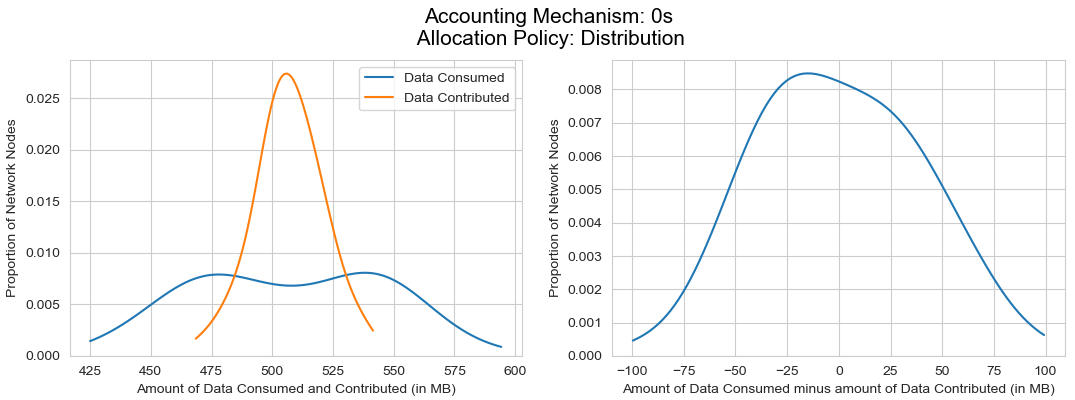
\includegraphics[scale=0.8]{Acc_0s_Dist.png} \\ 
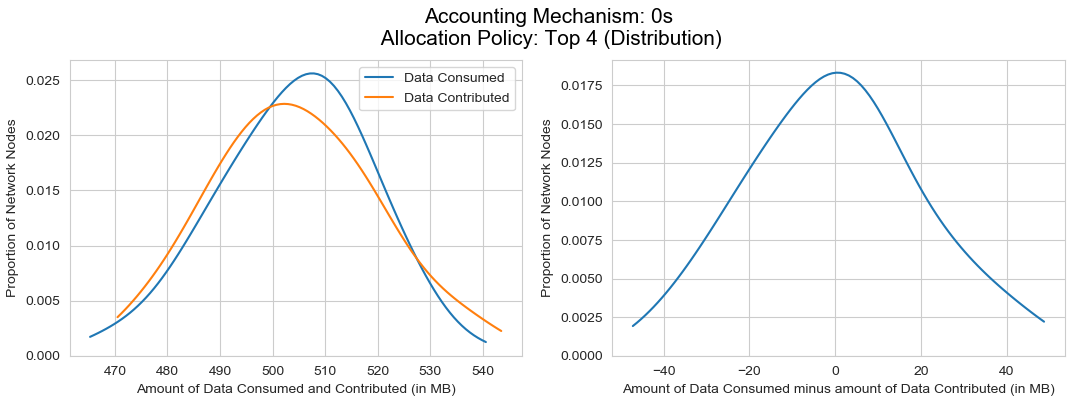
\includegraphics[scale=0.8]{Acc_0s_Top_4_Dist.png} \\
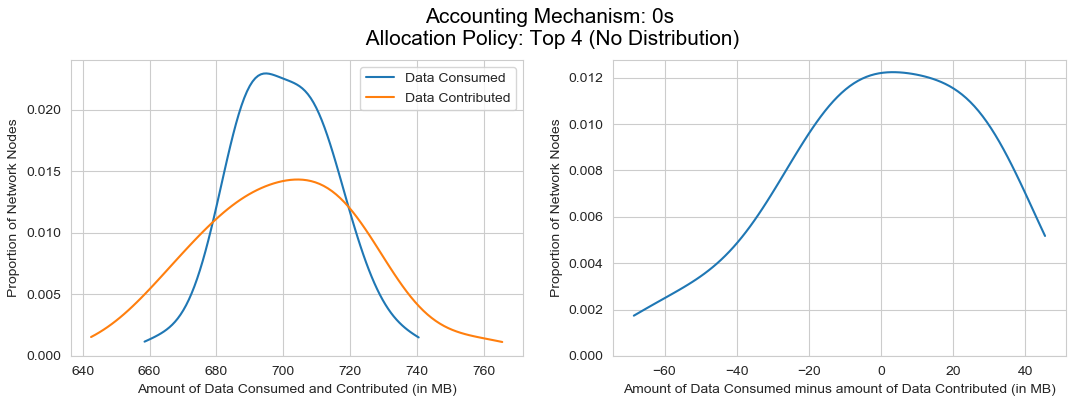
\includegraphics[scale=0.8]{Acc_0s_Top_4_No_Dist.png} \\
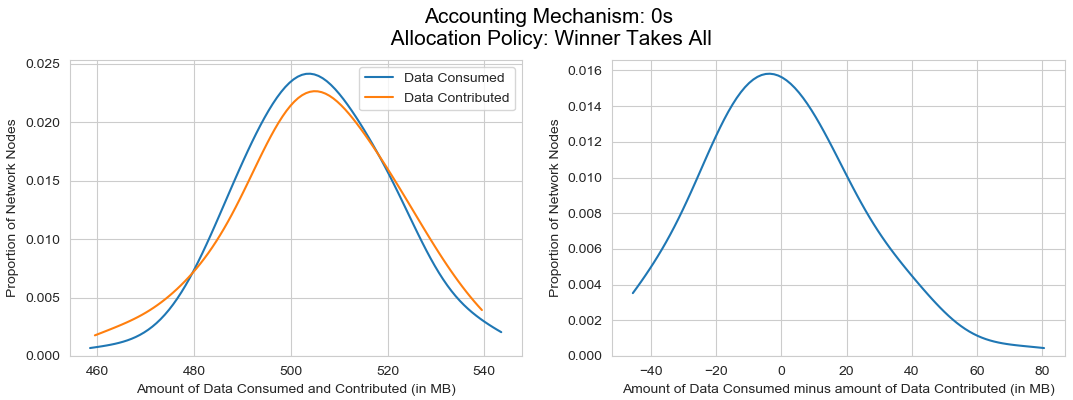
\includegraphics[scale=0.8]{Acc_0s_Winner.png} \\
\end{tabular}
\caption{Simulation values of the Interaction Model given $S^M_i(G_i,j)=0$.}
\label{fig:Acc_0s_Sim_Values}
\end{center}
\end{figure}

\begin{figure}[H]
\begin{center}
\begin{tabular}{c}
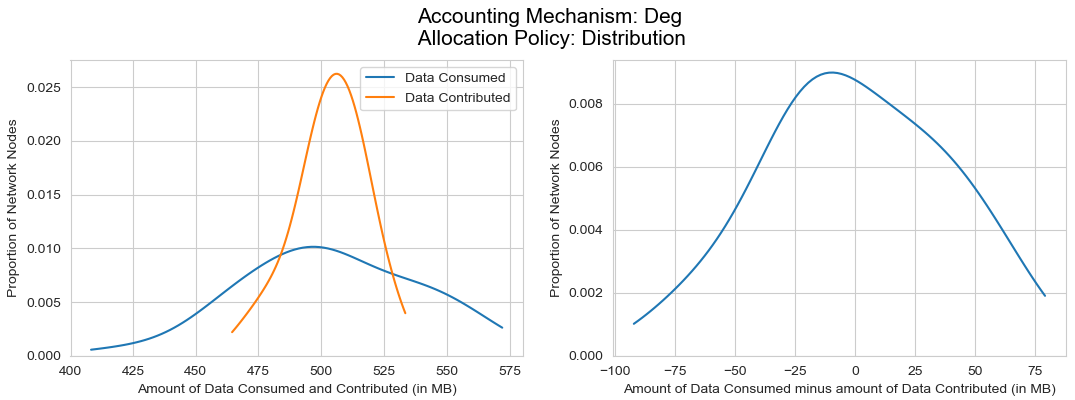
\includegraphics[scale=0.8]{Acc_Deg_Dist.png} \\
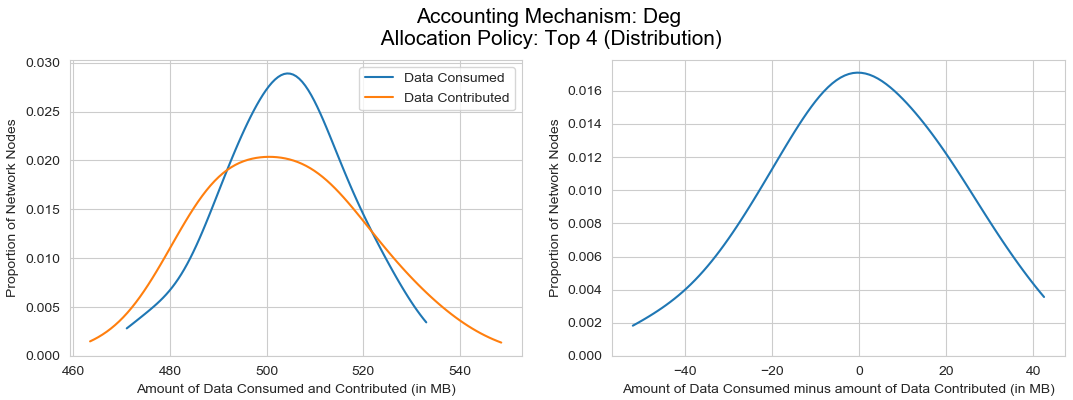
\includegraphics[scale=0.8]{Acc_Deg_Top_4_Dist.png} \\
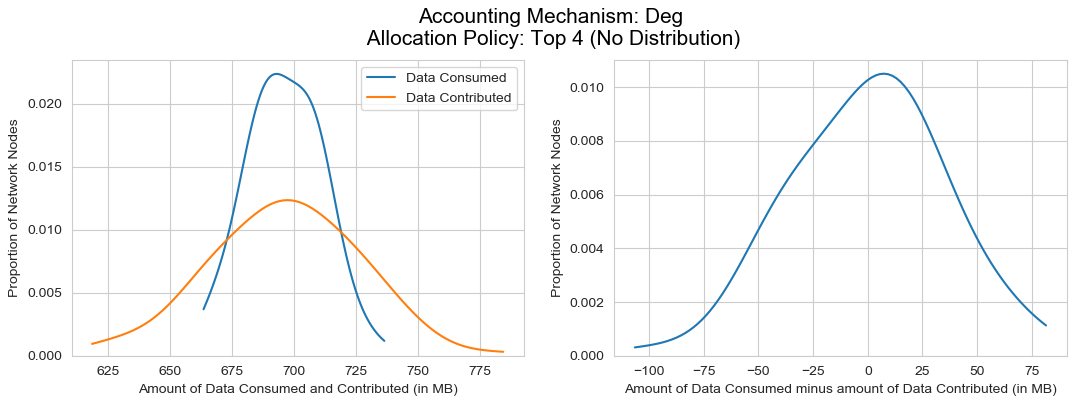
\includegraphics[scale=0.8]{Acc_Deg_Top_4_No_Dist.png} \\
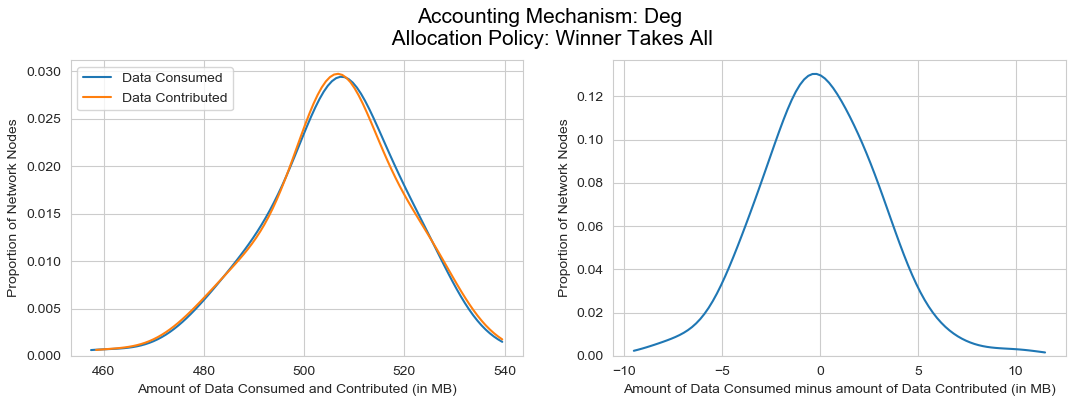
\includegraphics[scale=0.8]{Acc_Deg_Winner.png} \\
\end{tabular}
\caption{Simulation values of the Interaction Model given $S^{Deg}_i(G_i,j)$.}
\label{fig:Acc_Deg_Sim_Values}
\end{center}
\end{figure}

\begin{figure}[H]
\begin{center}
\begin{tabular}{c}
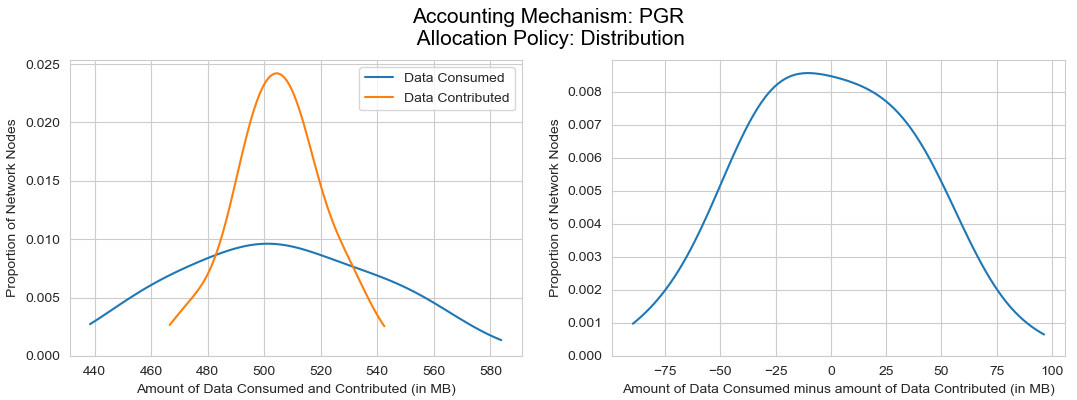
\includegraphics[scale=0.8]{Acc_PGR_Dist.png} \\
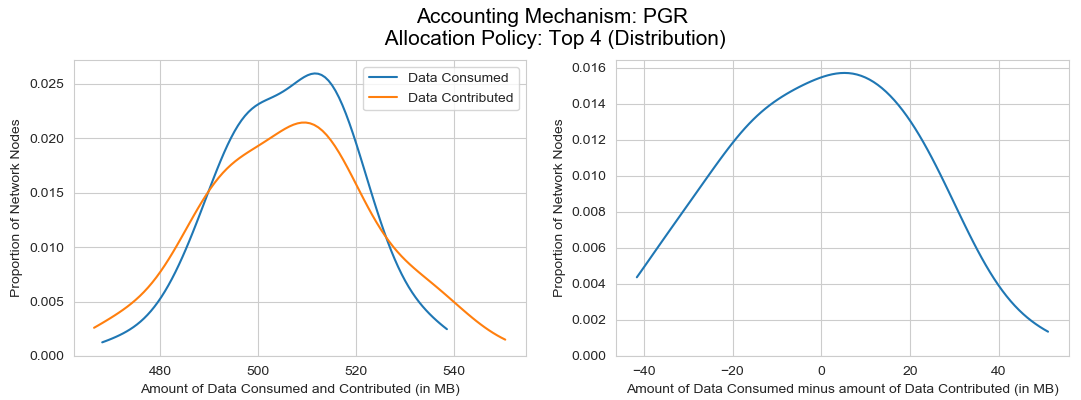
\includegraphics[scale=0.8]{Acc_PGR_Top_4_Dist.png} \\
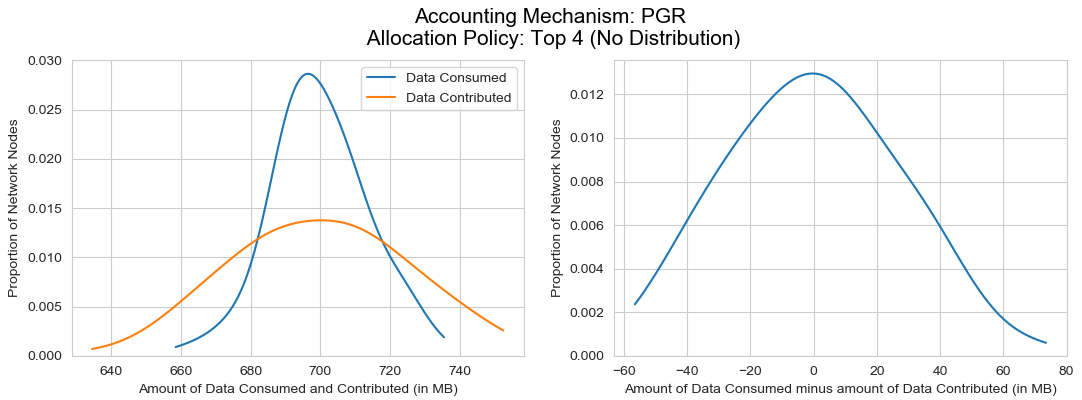
\includegraphics[scale=0.8]{Acc_PGR_Top_4_No_Dist.png} \\
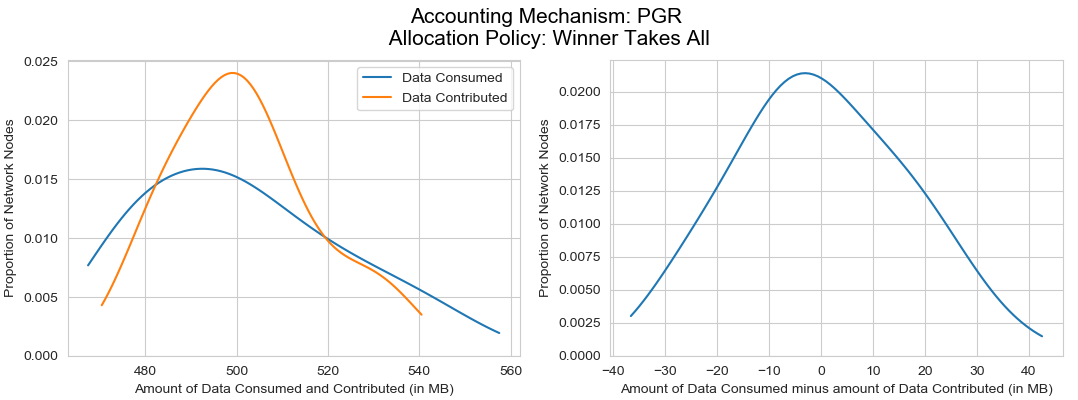
\includegraphics[scale=0.8]{Acc_PGR_Winner.png} \\
\end{tabular}
\caption{Simulation values of the Interaction Model given $S^{PGR}_i(G_i,j)$.}
\label{fig:Acc_PGR_Sim_Values}
\end{center}
\end{figure}


\noindent{}For the simplest accounting mechanism that assigns $0$'s to all nodes in the network, we find that the distribution policy leads to a rather wide-ranging distribution of net contributions made to the network, which implies that the distribution policy is not very effective in preventing or mitigating lazy freeriding. Additionally, we see that the distributions of contributions and consumption are quite different. This means the distribution policy leads to an somewhat inefficient distribution of data in the network and does not reward contributions effectively. The top-4 (distribution) policy does a much better job at preventing lazy freeriding than the distribution policy as we can see from the relatively small variance of the distribution of net consumption in the network. It also leads to a fairer distribution of data. The top-4 (no distribution) policy is even less effective at preventing lazy freeriding and facilitating a fair distribution of data. Lastly, we find that the winner-takes-all policy returns quite nice results for the distribution of net consumption with the exception of two outliers. The distributions of consumption and contribution are also not too different and we conclude that the best allocation policy for the all $0$s accounting mechanism is in fact the winner-takes-all policy. \vspace{1em}\\

\noindent{}For the degree accounting mechanism we find that the distribution policy is very ineffective at punishing freeriders and does not distribute data fairly at all. The top 4 policy without distribution performs equally badly, as can be seen from a rather larger variance in net contributions and unequal distributions of contribution and consumption. The top 4 policy with data distribution is much stronger in both regards with a relatively small variance in the net contributions and similar graphs on the left as well. However, the winner-takes-all policy is by far the best with a extremely small variance in net contributions and almost equal distributions of consumption and contribution. Hence the winner-takes-all policy again is the most effective both in terms of preventing lazy freeriding as well as in facilitating cooperativeness. \vspace{1em}\\

\noindent{}In the case of the personalised PageRank accounting mechanism we find that the distribution policy returns a distribution similar to the distributions we saw for different accounting mechanisms. The fact that the distribution policy always returns very similar distributions of data in the network lies in the fact that every node in the choice set is always served and only the amount the it receives varies depending on its accounting value. The same holds for the top 4 (distribution policy). Although we do observe some differences between its distributions. These may, however be attributed to the randomness of the simulation. As before, the winner-takes-all policy outperforms all other policies, both in preventing freeriding and in rewarding contributions. We note that in terms of rewarding contributions it is outperformed by the top-4 (distribution) policy, albeit by not too much. We conclude this section by noting that the experimental results support our hypothesis and that the winner-takes-all policy is a good choice for the upper interaction model.\vspace{1em}\\

\noindent{}We realise that the set of allocation policies that we investigate is rather limited and that there may be much better allocation policies out there. A possible superior alternative to the winner-takes-all policy could be given by 

\[
A_i(S_i^M(G_i),C_i):=\left\lbrace{} j\in{}C_i\,|\,S^M_i(G_i,j) > 0 \right\rbrace ,
\]

\noindent{}where every node in $A_i(S_i^M(G_i),C_i)$ receives

\[
\tilde{\omega}\cdot\frac{S^M_i(G_i,j)}{\sum\limits_{k\in{}C_i}S^M_i(G_i,k)}.
\]

\noindent{}The reason this allocation policy may be superior to the winner-takes-all policy is that it prevents large-scale sybil attacks, due to the fact that it only serves nodes with accounting values greater than $0$, and therefore sybil nodes will not be served as much. At the same time it does not restrict the distribution to a single node the way the winner-takes-all policy does. For time reasons we did not ffurther investigate this policy. \vspace{1em}\\

\noindent{}Recall that it was the goal of this chapter to define the cost and profit of a sybil attack and so far we have only covered the cost of a sybil attack in definition \ref{def:Sybil Attack Cost}. The reason we took this "detour" to discuss an interaction model and allocation policies is so that we could define the profit of a sybil attack, which we will do now with the upper results on allocation policies in mind.\vspace{1em}\\

 
\begin{definition}[Sybil Attack Profit]\ \\
\label{def:Sybil Attack Profit}
\noindent{}For simplicity of formula we relable $X_{ij}:=S^M_i(G_i,j)$ and define the random vectors $X_i:=(X_{i1},\ldots,X_{in})$ for $i\in{}V$. We define the random variable $Y_{ik}$ as the indicator function which is 1 if $X_{ik}\geq{}X_{ij}$ f.a. $j\in{}C_i$ and $k\in{}C_i$ and zero else. We then define $G'^{(1)}$ as the work graph after the attacker and their sybils have consumed the work they were elligible for after the attack. This continues round for round yielding work graphs $\left(G'^{(n)}\right)_{n\in\mathbb{N}}$. Then we define the expected amount of work node $j$ can consume after sybil attack $\sigma_j^n$ as 

\[
\omega_{+}^{n} = \sum\limits_{n\in\mathbb{N}}\tilde{\omega}\cdot\mathbb{E}\left[\sum\limits_{i\in{}V'\backslash\lbrace{}j,s_{j1},\ldots,s_{j|S|}\rbrace}\sum\limits_{l=1}^{|S|}Y'^{(n)}_{is_{jl}} + Y'^{(n)}_{ij}\right].
\]
\noindent{}At this point, our assumption of an infinite network from \ref{subsec:Interaction Model} comes into play. Without this assumption there would be a possibility that a node $j$ with $S^M_i(G_i,j)=0$ may be served by node $i$ in a particular round, if it is the only node in $i$'s choice set. Therefore, we find that for any node that queries another node with probability $q$ in every round, the upper sum will be infinite. In order to curb this, assumed that while $V_i$ is obviously always finite, there are infinite nodes $u\in{}V$ outside of $i$'s subjective work graph, all with $S^M_i(G_i,u)=0$ that will make queries to other nodes following the same paradigm as above. By this logic the choice set $C_i$ will be of infinite size in every round and the probability of $j$ being served in any given round is arbitrarily small. This results in the sum above being finite for any node in the network that does not "cheat".
\end{definition}

\noindent{}Note that this specification has been completely neglected in the existing literature. In their research Seuken \& Parkes have not specified the values $\omega_{+}^{n}$ and $\omega_{-}^{n}$. However, it is an important one to make, as according to their definition it would always hold $\omega_{+}^n=\infty$. At least for most of the allocation policies discussed in section \ref{chap:Mathematical Framework for Accounting Mechanisms} and therefore any sybil attack would be strongly beneficial with respect to definition \ref{def:Sybil Attack Benefit}. They kept their definition of $\omega_{+}^n$ very vague, referring to it as "the amount of work that agent j or any
of its sybils will be able to consume", but did not specify a time frame \cite{On the Sybil-Proofness of Accounting Mechanisms}. The same applies to $\omega_{-}^n$.\vspace{1em}\\

\noindent{}Otte et al. (2016) solve this problem by assuming an allocation policy called the \textit{strict winner-takes-all policy}, which serves the highest ranking node in the choice set, just like the winner-takes-all policy. However, if all nodes in the choice set have the same accounting values then the strict winner-takes-all policy doesn't serve anyone. We dismiss this allocation policy for the same reasons we disagree with the banning policy in \ref{ex:Banning Policy}, namely that it limits distribution of data in the network.\vspace{1em}\\ 

\noindent{}Now that we have definitions for both the cost and profit of a sybil attack we return to the definition of the benefit of a sybil attack, defined above in definition \ref{def:Sybil Attack Benefit}. Again, we say that a sybil attack is 

\begin{itemize}
\item[] {\bf Strongly Beneficial} if $\omega^n_{+}>0$ and $\omega^n_{-}=0$ or if $\lim\limits_{n\rightarrow\infty}\frac{\omega^n_{+}}{\omega^n_{-}}=\infty$,
\item[] {\bf Weakly Beneficial} if $\omega^n_{+}>0$ and $\omega^n_{-}>0$ and $\exists c>0:\,\,\lim\limits_{n\rightarrow\infty}\frac{\omega^n_{+}}{\omega^n_{-}}\geq{}c$.
\end{itemize}

\noindent{}We inverse these points to introduce sybil resistance.

\begin{definition}[Sybil Resistance]\ \\
\label{def:Sybil Resistance}
\noindent{}Let $j$ be a malicious node perpetrating a sybil attack $\sigma_j^n$ on the work graph $G$, resulting in work graph $G'$. Here $n$ is variable. Now let $\omega_{-}^{n}>0$ denote the cost of the sybil attack $\sigma_j^n$, according to definition \ref{def:Sybil Attack Cost} and let $\omega_{+}^n$ be the sybil attack profit defined in definition \ref{def:Sybil Attack Profit}. Then we call a pair of accounting mechanism and allocation policy $(S^M_i,A_i)$
\begin{itemize}
\item {\bf resistant against strongly beneficial sybil attacks} if 
\[
\forall{}j\in{}V_i\backslash{}\left\lbrace{}i\right\rbrace \forall (\sigma^n_j)_{n\in\mathbb{N}}\,\exists{}c>0:\,\,\lim\limits_{n\rightarrow\infty}\frac{\omega^n_{+}}{\omega^n_{-}}\leq{}c,
\]
\item {\bf resistant against weakly beneficial sybil attacks} if 
\[
\forall{}j\in{}V_i\backslash{}\left\lbrace{}i\right\rbrace \forall (\sigma^n_j)_{n\in\mathbb{N}}:\,\,\lim\limits_{n\in\mathbb{N}}\frac{\omega^n_{+}}{\omega^n_{-}}=0.
\]
\end{itemize}
\end{definition}

\noindent{}Note that sybil-proofness against weakly beneficial attacks is extremely restrictive and very hard to obtain by any form of accounting mechanism, while sybil-proofness against strongly beneficial attacks is easier to achieve and by our standards sufficient for the maintainance of a (mostly) cooperative, functioning network. The reason for this is that while an attacker can launch a sybil attack that returns a multiple of its investment, the idea is that in order for an attacker to leach infinite data, they also have to share infinite data. This means that any form of sybil attack will require some input into the network. No attacker can simply demand all resources in the network, leading to a complete shutdown. Instead, a weakly beneficial sybil attack still stimulates a network enough to maintain its existence. \vspace{1em}\\

\noindent{}Now that we have determined the cost and profit of sybil attacks, we should be able to determine for any pair $(S^M_i,A_i)$ whether it is sybil-resistant or not. However, we remark that due to the probabilistic nature of the the sum in \ref{def:Sybil Attack Profit} it is  impossible to compute for any generic setting making it impossible to determine how effective a sybil attack actually is. We need to renew the upper definitions in a way that makes them more easily computable. \vspace{1em}\\

\noindent{}This brings us to the next section where we reintroduce the profit and cost of sybil attacks in terms of accounting values, instead of work. \vspace{1em}\\


\section{Redefining Cost \& Profit in Terms of Accounting Values}
\label{sec:Cost & Profit in Terms of Accounting Values}
\noindent{}Recall that accounting mechanisms were there to determine the standing of a node in the network and capture how much data an agent is elligible to consume. In a sybil attack it is the goal of the attacker to increase the accounting values of one or more nodes in the sybil region from the perspective of as many honest nodes as possible to be able to consume larger amounts of data from the network. \vspace{1em}\\

\noindent{}In order for us to be able to gauge how profitable an attack is, we introduce another pair of definitions of sybil attack rewards, which we denote $\omega_{+}^{n}$(rep) and $\omega_{-}^{n}$(rep). For uniformity we relabel the former definitions of cost and profit as $\omega_{+}^{n}$(work) and $\omega_{-}^{n}$(work). \vspace{1em}\\ 

\noindent{}In this setting, one might define the reward of an attack $\sigma_j^n$ in terms of accounting mechanisms by the aggregate of accounting values all sybil nodes (including $j$) have collectively obtained through the attack. 

\[
\sum\limits_{i\in{}V'\backslash\left\lbrace{}j,s_{j1}\ldots{}s_{jn}\right\rbrace}\sum\limits_{s\in\left\lbrace{}j,s_{j1}\ldots{}s_{jn}\right\rbrace}S^M_i(G'_i,s).
\]

\noindent{}And we obtain the following definition of sybil attack profit.\vspace{1em}\\

\begin{definition}[Sybil Attack Profit in Terms of Accounting Values]\ \\
\label{def:Sybil Attack Profit (rep)}
\noindent{}Given an objective and a subjective work graph $G:=(V,E,w)$, $G_i:=(V_i,E_i,w_i)$, let $\sigma_j^n$ be a sybil attack of size $n\in\mathbb{N}$ with Sybil region $S=\left\lbrace{}s_{j1},\ldots,s_{jn}\right\rbrace$, whereby $n$ is not fixed. Take $G':=(V',E',w')$ and $G_i':=(V_i',E_i',w_i')$ as defined above. We define $\omega_{+}^{n}$(rep) as the aggregate of accounting values that nodes in the sybil region collectively gain after it has carried out its attack. We obtain

\[
\omega_{+}^{n}({\rm rep}) = \sum\limits_{i\in{}V'\backslash\lbrace{}j,s_1,\ldots,s_n\rbrace}\sum\limits_{s\in\lbrace{}j,s_1,\ldots,s_n\rbrace}S^M_i(G_i',s).
\]
% - \sum\limits_{i\in{}V\backslash\lbrace{}j\rbrace}S^M_j(G_i,C_i)
\end{definition}

\noindent{}We now need to define $\omega^{n}_{-}$(rep). Just as in definition \ref{def:Sybil Attack Profit (rep)} this value needs to be equivalent to the earlier defined $\omega_{-}^{n}$(work), but in terms of accounting values. The reasoning for the definition of $\omega_{-}^{n}$(work) above was that we were trying to capture the amount of work invested into the network by a sybil attacker, i.e. the aggregate of the weights of the attack edges. In terms of accounting values, we can define this concept as the aggregated accounting values a sybil attacker has "earned" through their honest work, invested into the network. \vspace{1em}\\

\begin{definition}[Sybil Attack Cost in Terms of Accounting Values]\ \\
\label{def:Sybil Attack Cost (rep)}
\noindent{}Given an objective and a subjective work graph $G:=(V,E,w)$, $G_i:=(V_i,E_i,w_i)$, let $\sigma_j^n$ be a sybil attack of size $n\in\mathbb{N}$ with Sybil region $S=\left\lbrace{}s_{j1},\ldots,s_{jn}\right\rbrace$, whereby $n$ is not fixed. Take $G':=(V',E',w')$ and $G_i':=(V_i',E_i',w_i')$ as defined above. \vspace{1em}\\

\noindent{}Now we introduce a third graph $G''=(V'',E'',w'')$ where $V''=V$ and $w'':V\times{}V\rightarrow\mathbb{R}$ with $w''(u,v)=w(u,v)$ f.a. $u,v\in{}V\backslash\left\lbrace{}j\right\rbrace$ and $w''(u,j)=\sum\limits_{s\in{}S\cup\left\lbrace{}j\right\rbrace}w'(u,s)$ as well as $w''(j,u)=\sum\limits_{s\in{}S\cup\left\lbrace{}j\right\rbrace}w'(s,j)$. Graphically, this means that we "collapse" all sybil nodes into a single node which we will label $j$ again and all incoming and all outgoing edges from any sybil node into the honest region of the graph, are attached to $j$ in $G''$. \vspace{1em}\\

\begin{figure}[H]
\begin{center}
\includegraphics[scale=0.9]{"Cost Rep(1)".PNG} 
\includegraphics[scale=0.9]{"Cost Rep(2)".PNG} 
\includegraphics[scale=0.9]{"Cost Rep(3)".PNG}
\end{center}
\label{fig:Example of Collapsing a Sybil Region}
\caption{Example of Collapsing a Sybil Region}
\end{figure}

\noindent{}The point is that the aggregate of accounting values that the sybil attacker has gained should be compared to the accounting values that they're actually entitled to based on the actual work performed, i.e. the attack edges. All edges that do not enter or leave the sybil region are therefore disregarded and any increase in reputation that the sybil attackers may gain through the sybil-internal edges is dropped. In formula we then obtain the following value of sybil attack cost \vspace{1em}\\

\[
\omega_{-}^{n}(rep) = \sum_{i\in{}V''\backslash\lbrace{}j\rbrace}S^M_i(G_i'',j).
\]

\end{definition}

\noindent{}We should mention here that we keep the same definitions of sybil attack benefit and sybil resistance as in definitions \ref{def:Sybil Attack Benefit} and \ref{def:Sybil Resistance} in both cases of sybil attack profit and cost. And we call sybil attacks strongly and weakly beneficial in terms of accounting values and in terms of work. \vspace{1em}\\